% You should title the file with a .tex extension (hw1.tex, for example)
\documentclass[11pt]{article}

\usepackage{amsmath}
\usepackage{amssymb}
\usepackage{fancyhdr}
\usepackage{listings}
\usepackage{color}
\usepackage{graphicx}
\graphicspath{ {images/} }
\usepackage{hyperref}
\usepackage{mathtools}

\definecolor{dkgreen}{rgb}{0,0.6,0}
\definecolor{gray}{rgb}{0.5,0.5,0.5}
\definecolor{mauve}{rgb}{0.58,0,0.82}

\lstset{frame=tb,
  language=Java,
  aboveskip=3mm,
  belowskip=3mm,
  showstringspaces=false,
  columns=flexible,
  basicstyle={\small\ttfamily},
  numbers=none,
  numberstyle=\tiny\color{gray},
  keywordstyle=\color{blue},
  commentstyle=\color{dkgreen},
  stringstyle=\color{mauve},
  breaklines=true,
  breakatwhitespace=true,
  tabsize=3
}

\oddsidemargin0cm
\topmargin-2cm     %I recommend adding these three lines to increase the 
\textwidth16.5cm   %amount of usable space on the page (and save trees)
\textheight23.5cm  

\newcommand{\question}[2] {\vspace{.25in} \hrule\vspace{0.5em}
\noindent{\bf #1: #2} \vspace{0.5em}
\hrule \vspace{.10in}}
\renewcommand{\part}[1] {\vspace{.10in} {\bf (#1)}}

\newcommand{\myname}{Chang-Hyun Mungai}
\newcommand{\myhwnum}{Behavioral Notes}

\setlength{\parindent}{0pt}
\setlength{\parskip}{5pt plus 1pt}
 
\pagestyle{fancyplain}
\lhead{\fancyplain{}{\textbf{\myhwnum}}}      % Note the different brackets!

\begin{document}

\medskip                        % Skip a "medium" amount of space
                                % (latex determines what medium is)
                                % Also try: \bigskip, \littleskip

\thispagestyle{plain}
\begin{center}                  % Center the following lines
{\Large Behavioral} \\
\end{center}

\question{General}

Identify common communication patterns between objects and realize these patterns

\question{Chain of Responsibility}

\begin{itemize}
  \item Definition/Use

  \begin{itemize}
    \item command objects are handled or passed on to other objects by logic-containing processing objects
    \item avoid coupling the sender of a request to its receiver by giving more than one object a chance to handle the request
  \end{itemize}

  \item Structure

  \begin{itemize}
    \item 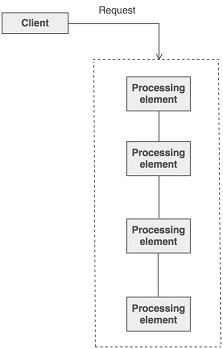
\includegraphics{chain_of_responsibility_2}
    \item 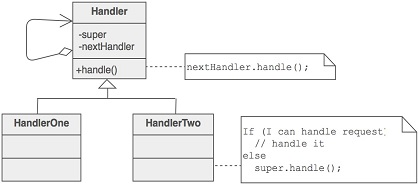
\includegraphics{chain_of_responsibility}
  \end{itemize}

  \item Notes

  \begin{itemize}
    \item base class maintains a next pointer
    \item if the request needs to be "passed on", then the derived class "calls back" to the base class, which delegates to the "next" pointer
  \end{itemize}

\end{itemize}

\question{Command}

\begin{itemize}
  \item Definition/Use

  \begin{itemize}
    \item command objects encapsulate an action and its parameters
    \item Need to issue requests to objects without knowing anything about the operation being requested or the receiver of the request
    \item separation provides flexibility in the timing and sequencing of commands
    \item command objects can be thought of as "tokens",created by one client that knows what need to be done, passed to another client that has the resources for doing it
  \end{itemize}

  \item Structure

  \begin{itemize}
    \item 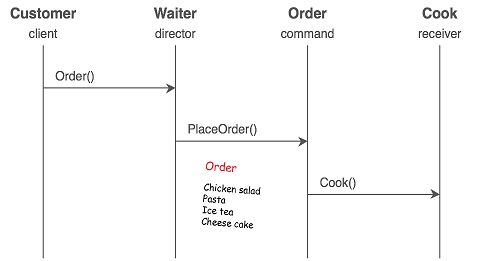
\includegraphics{Command_example}
  \end{itemize}

  \item Notes

  \begin{itemize}
    \item define a Command interface with a method signature like execute()
  \end{itemize}

\end{itemize}

\question{Interpreter}

\begin{itemize}
  \item Definition/Use

  \begin{itemize}
    \item implement a specialized computer language to rapidly solve a specific set of problems
    \item map a domain to a language, the language to a grammar, and the grammar to a hierarchical object  \item oriented design
  \end{itemize}

  \item Structure

  \begin{itemize}
    \item 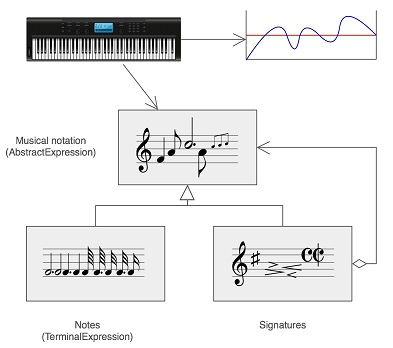
\includegraphics{Interpreter_example}
  \end{itemize}

  \item Notes

  \begin{itemize}
    \item the pattern doesn't address parsing. When the grammar is very complex, other techniques (such as a parser) are more appropriate
  \end{itemize}

\end{itemize}

\question{Iterator}

\begin{itemize}
  \item Definition/Use

  \begin{itemize}
    \item iterators are used to access the elements of an aggregate object sequentially without exposing its underlying representation
    \item need to "abstract" the traversal of wildly different data structures so that algorithms can be defined that are capable of interfacing with each transparently
  \end{itemize}

  \item Structure

  \begin{itemize}
    \item 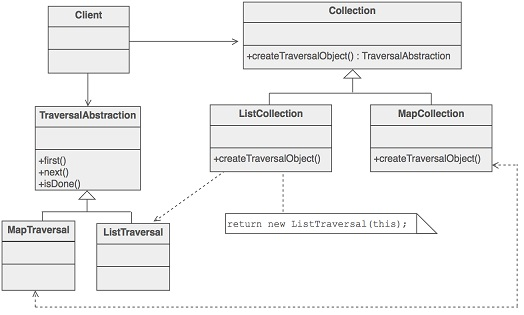
\includegraphics{Iterator-diagram}
  \end{itemize}

  \item Notes

  \begin{itemize}
    \item 

\begin{lstlisting}
clients use the first(), is_done(), next(), and current_item() protocol to access the elements of the collection class
\end{lstlisting}

  \end{itemize}

\end{itemize}

\question{Mediator}

\begin{itemize}
  \item Definition/Use

  \begin{itemize}
    \item provides a unified interface to a set of interfaces in a subsystem
    \item promotes loose coupling by keeping objects from referring to each other explicitly
  \end{itemize}

  \item Structure

  \begin{itemize}
    \item 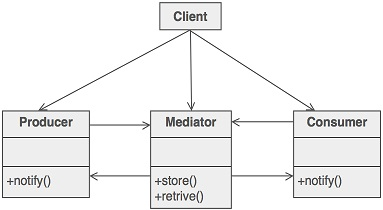
\includegraphics{Mediator}
    \item 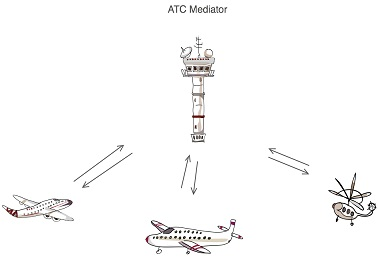
\includegraphics{Mediator_example}
  \end{itemize}

  \item Notes

  \begin{itemize}
    \item be careful not to create a "controller" or "god" object
  \end{itemize}

\end{itemize}

\question{Memento}

\begin{itemize}
  \item Definition/Use

  \begin{itemize}
    \item provides the ability to restore an object to its previous state (rollback)
    \item pattern defines three distinct roles

    \begin{itemize}
      \item originator : the object that knows how to save itself
      \item caretaker : the object that knows why and when the originator needs to save and restore itself
      \item memento : the lock box that is written and read by the originator, and shepherded by the caretaker
    \end{itemize}

  \end{itemize}

  \item Structure

  \begin{itemize}
    \item 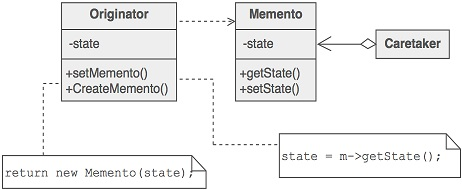
\includegraphics{Memento}
  \end{itemize}

  \item Notes

  \begin{itemize}
    \item identify the roles of “caretaker” and “originator”
  \end{itemize}

\end{itemize}

\question{Observer(Publish/Subscribe or Event Listener)}

\begin{itemize}
  \item Definition/Use

  \begin{itemize}
    \item objects register to observe an event that may be raised by another object
    \item defines a one  \item to  \item many relationship so that when one object changes state, the others are notified and updated automatically
  \end{itemize}

  \item Structure

  \begin{itemize}
    \item 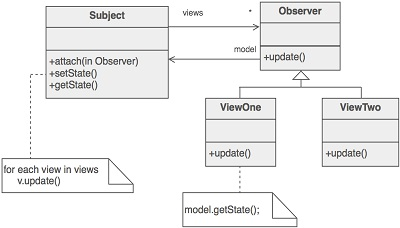
\includegraphics{Observer}
    \item 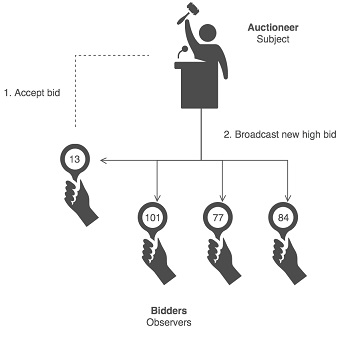
\includegraphics{Observer_example}
  \end{itemize}

  \item Notes

  \begin{itemize}
    \item subject broadcasts events to all registered observers
  \end{itemize}

\end{itemize}

\question{State}

\begin{itemize}
  \item Definition/Use

  \begin{itemize}
    \item a clean way for an object to partially change its type at runtime
    \item a monolithic object's behavior is a function of its state
  \end{itemize}

  \item Structure

  \begin{itemize}
    \item 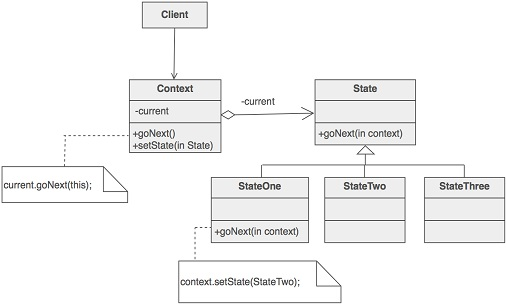
\includegraphics{State}
    \item 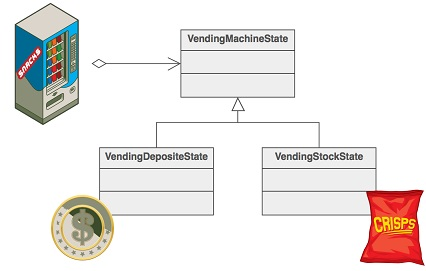
\includegraphics{State_example}
  \end{itemize}

  \item Notes

  \begin{itemize}
    \item pattern does not specify where the state transitions will be defined

    \begin{itemize}
      \item the "context" object
      \item each individual State derived class

      \begin{itemize}
        \item advantage is ease of adding new State derived classes
        \item disadvantage is each State derived class has knowledge of (coupling to) its siblings, which introduces dependencies between subclasses
      \end{itemize}

    \end{itemize}

  \end{itemize}

\end{itemize}

\question{Strategy}

\begin{itemize}
  \item Definition/Use

  \begin{itemize}
    \item algorithms can be selected on the fly
    \item defines a set of algorithms that can be used interchangeably
  \end{itemize}

  \item Structure

  \begin{itemize}
    \item 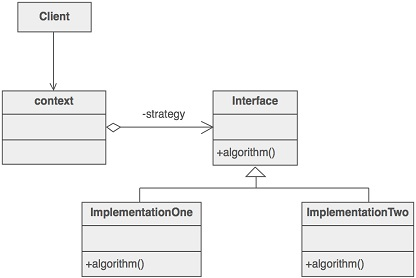
\includegraphics{Strategy}
  \end{itemize}

  \item Notes

  \begin{itemize}
    \item identify an algorithm (i.e. a behavior) that the client would prefer to access through a "flex point"
  \end{itemize}

\end{itemize}

\question{Template method}

\begin{itemize}
  \item Definition/Use

  \begin{itemize}
    \item describes the program skeleton of a program
    \item component designer decides which steps of an algorithm are invariant (or standard), and which are variant (or customizable)
  \end{itemize}

  \item Structure

  \begin{itemize}
    \item 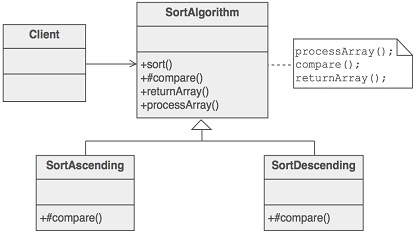
\includegraphics{Template_Method}
    \item 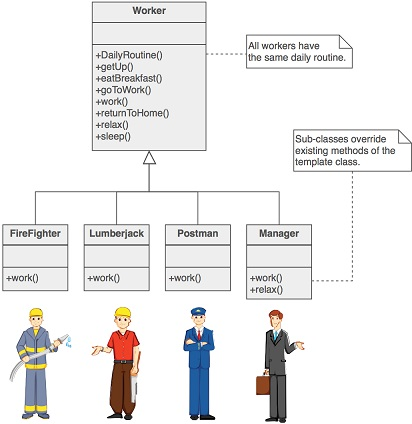
\includegraphics{Template_method_example}
  \end{itemize}

  \item Notes

  \begin{itemize}
    \item examine the algorithm, and decide which steps are standard and which steps are peculiar to each of the current classes
  \end{itemize}

\end{itemize}

\question{Visitor}

\begin{itemize}
  \item Definition/Use

  \begin{itemize}
    \item a way to separate an algorithm from an object
  \end{itemize}

  \item Structure

  \begin{itemize}
    \item 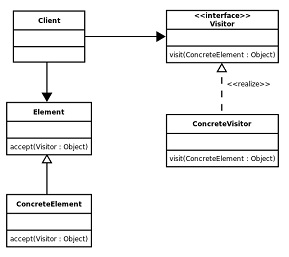
\includegraphics{Visitor}
    \item 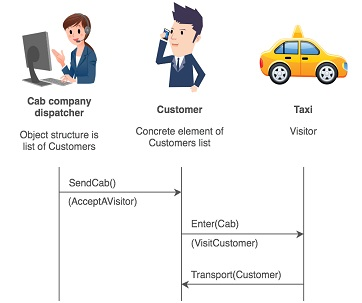
\includegraphics{Visitor_example}
  \end{itemize}

  \item Example

  \begin{itemize}
    \item
\begin{lstlisting}
public interface CharacterVisitor {

  public void visit(char aChar);

}

public class MyString {

// ... other methods, fields

  // Our main implementation of the visitor pattern
  public void foreach(CharacterVisitor aVisitor) {
    int length = this.length();
    // Loop over all the characters in the string
    for (int i = 0; i < length; i++) {
      // Get the current character, and let the visitor visit it.
      aVisitor.visit(this.getCharAt(i));
    }
  }

// ... other methods, fields

}// end class MyString

public class MyStringPrinter implements CharacterVisitor {

  // We have to implement this method because we're implementing the CharacterVisitor
  // interface
  public void visit(char aChar) {
    // All we're going to do is print the current character to the standard output
    System.out.print(aChar);
  }

  // This is the method you call when you want to print a string
  public void print(MyString aStr) {
    // we'll let the string determine how to get each character, and
    // we already defined what to do with each character in our
    // visit method.
    aStr.foreach(this);
  }

} // end class MyStringPrinter
\end{lstlisting}
  \end{itemize}

  \item Notes

  \begin{itemize}
    \item if you have and will always have only one visitor, you'd rather implement the composite pattern
  \end{itemize}

\end{itemize}

\question{Comparison}

\begin{itemize}
  \item chain of Responsibility, command, mediator, and observer, address how you can decouple senders and receivers, but with different trade  \item offs

  \begin{itemize}
    \item chain of Responsibility passes a sender request along a chain of potential receivers
  \end{itemize}

  \item command and memento act as magic tokens to be passed around and invoked at a later time

  \begin{itemize}
    \item in command, the token represents a request
    \item in memento, it represents the internal state of an object at a particular time
    \item polymorphism is important to command, but not to memento because its interface is so narrow that a memento can only be passed as a value
  \end{itemize}

\end{itemize}

\end{document}

